\zchapter{Your Account}\label{SetupAccount}

% How to actually make an account. Most Freshers never do this :-(

%\begin{mdframed}

\section{Getting it}

\textsc{signing up at the O'Day stall is the first step to gaining access to all of UCC's services. The next step is visiting the clubroom to create an account.}

Your UCC account is \emph{the most} important thing you can have as a member.
The account lets you log into any of our clubroom machines, user servers, wireless network, online drink and snack machines, and more.
It also provides you with an email address that we may use to communicate with you.

Once you're at the clubroom and ready to create an account, ask around for a member who can set up your account. Members in UCC are kind and will let you know who can help if you ask. You'll get to choose your own user name and a password. The person who sets up your account will also show you around the clubroom and how to operate our drink and snack machines.

Now that you have an account, you can use it to log into any of our clubroom machines. If you want to log onto one of our servers, you'll need to use the SSH program. If you're having trouble, just ask someone in the clubroom --- we don't \pun{byte}!

Changing your UCC password can either be done by Ctrl-Alt-Del on a windows machine or using the command \shell{passwd} on a Linux/Unix machine.
Accessing the UCC WiFi network can be a bit tricky (particularly on Windows machines). Ask someone if you need help, or refer to \url{http://wiki.ucc.asn.au/Wifi}

%\end{mdframed}

%\pagebreak

%\begin{mdframed}

\section{SSH for the Greater Good}

SSH is a program that lets you remotely access UCC's servers. These can be used for almost anything (legal) you can imagine; programming, website hosting, file storage, IRC chatting, dispensing drinks, and many more things.

%The easiest way to use SSH is from a Linux clubroom desktop. Simply open a "terminal" application, type \shell{ssh username@ssh.ucc.asn.au} and enter your password. %It should look like Figure \ref{ssh.png}.

From a windows computer, open a program called "PuTTy" (or "KiTTy"). Enter the address \shell{username@ssh.ucc.asn.au} and click "Open". You can SSH from home using the same address. %See Figure \ref{putty.png}.

%Once you are logged in, a good way to start is running "irssi -c irc" and then typing "/join \#ucc". The interface of irssi takes some getting used to, but when combined with "screen" (ask someone for help) it is a powerful weapon for procrastination.

%You don't have to be in the UCC clubroom to use SSH! Simply use \shell{username@ssh.ucc.asn.au} as the address to connect to.

%\end{mdframed}

%\begin{mdframed}


%\begin{figure}[H]
%	\centering
%	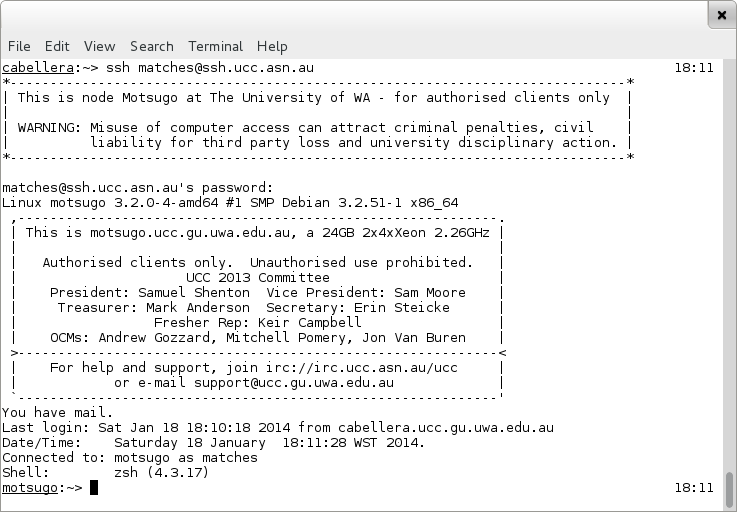
\includegraphics[width=1.0\textwidth]{figures/ssh.png}
%	\caption{SSH from Linux} 
%	\label{ssh.png}
%\end{figure}

%\begin{figure}[H]
%	\centering
%	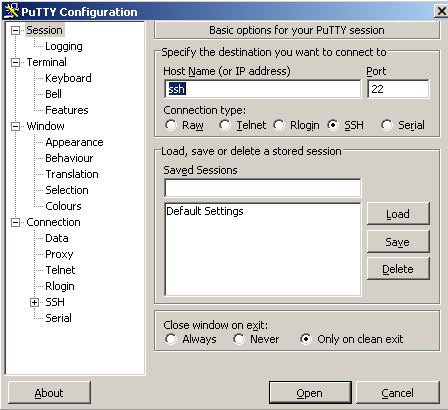
\includegraphics[width=0.5\textwidth]{figures/putty.png}
%	\caption{Use PuTTY to SSH. Just press "Open"} 
%	\label{putty.png}
%\end{figure}

%\end{mdframed}
